\documentclass[]{article}
\usepackage{lmodern}
\usepackage{amssymb,amsmath}
\usepackage{ifxetex,ifluatex}
\usepackage{fixltx2e} % provides \textsubscript
\ifnum 0\ifxetex 1\fi\ifluatex 1\fi=0 % if pdftex
  \usepackage[T1]{fontenc}
  \usepackage[utf8]{inputenc}
\else % if luatex or xelatex
  \ifxetex
    \usepackage{mathspec}
  \else
    \usepackage{fontspec}
  \fi
  \defaultfontfeatures{Ligatures=TeX,Scale=MatchLowercase}
\fi
% use upquote if available, for straight quotes in verbatim environments
\IfFileExists{upquote.sty}{\usepackage{upquote}}{}
% use microtype if available
\IfFileExists{microtype.sty}{%
\usepackage{microtype}
\UseMicrotypeSet[protrusion]{basicmath} % disable protrusion for tt fonts
}{}
\usepackage[margin=1in]{geometry}
\usepackage{hyperref}
\hypersetup{unicode=true,
            pdftitle={MLflow with R},
            pdfauthor={Javier Luraschi},
            pdfborder={0 0 0},
            breaklinks=true}
\urlstyle{same}  % don't use monospace font for urls
\usepackage{color}
\usepackage{fancyvrb}
\newcommand{\VerbBar}{|}
\newcommand{\VERB}{\Verb[commandchars=\\\{\}]}
\DefineVerbatimEnvironment{Highlighting}{Verbatim}{commandchars=\\\{\}}
% Add ',fontsize=\small' for more characters per line
\usepackage{framed}
\definecolor{shadecolor}{RGB}{248,248,248}
\newenvironment{Shaded}{\begin{snugshade}}{\end{snugshade}}
\newcommand{\AlertTok}[1]{\textcolor[rgb]{0.94,0.16,0.16}{#1}}
\newcommand{\AnnotationTok}[1]{\textcolor[rgb]{0.56,0.35,0.01}{\textbf{\textit{#1}}}}
\newcommand{\AttributeTok}[1]{\textcolor[rgb]{0.77,0.63,0.00}{#1}}
\newcommand{\BaseNTok}[1]{\textcolor[rgb]{0.00,0.00,0.81}{#1}}
\newcommand{\BuiltInTok}[1]{#1}
\newcommand{\CharTok}[1]{\textcolor[rgb]{0.31,0.60,0.02}{#1}}
\newcommand{\CommentTok}[1]{\textcolor[rgb]{0.56,0.35,0.01}{\textit{#1}}}
\newcommand{\CommentVarTok}[1]{\textcolor[rgb]{0.56,0.35,0.01}{\textbf{\textit{#1}}}}
\newcommand{\ConstantTok}[1]{\textcolor[rgb]{0.00,0.00,0.00}{#1}}
\newcommand{\ControlFlowTok}[1]{\textcolor[rgb]{0.13,0.29,0.53}{\textbf{#1}}}
\newcommand{\DataTypeTok}[1]{\textcolor[rgb]{0.13,0.29,0.53}{#1}}
\newcommand{\DecValTok}[1]{\textcolor[rgb]{0.00,0.00,0.81}{#1}}
\newcommand{\DocumentationTok}[1]{\textcolor[rgb]{0.56,0.35,0.01}{\textbf{\textit{#1}}}}
\newcommand{\ErrorTok}[1]{\textcolor[rgb]{0.64,0.00,0.00}{\textbf{#1}}}
\newcommand{\ExtensionTok}[1]{#1}
\newcommand{\FloatTok}[1]{\textcolor[rgb]{0.00,0.00,0.81}{#1}}
\newcommand{\FunctionTok}[1]{\textcolor[rgb]{0.00,0.00,0.00}{#1}}
\newcommand{\ImportTok}[1]{#1}
\newcommand{\InformationTok}[1]{\textcolor[rgb]{0.56,0.35,0.01}{\textbf{\textit{#1}}}}
\newcommand{\KeywordTok}[1]{\textcolor[rgb]{0.13,0.29,0.53}{\textbf{#1}}}
\newcommand{\NormalTok}[1]{#1}
\newcommand{\OperatorTok}[1]{\textcolor[rgb]{0.81,0.36,0.00}{\textbf{#1}}}
\newcommand{\OtherTok}[1]{\textcolor[rgb]{0.56,0.35,0.01}{#1}}
\newcommand{\PreprocessorTok}[1]{\textcolor[rgb]{0.56,0.35,0.01}{\textit{#1}}}
\newcommand{\RegionMarkerTok}[1]{#1}
\newcommand{\SpecialCharTok}[1]{\textcolor[rgb]{0.00,0.00,0.00}{#1}}
\newcommand{\SpecialStringTok}[1]{\textcolor[rgb]{0.31,0.60,0.02}{#1}}
\newcommand{\StringTok}[1]{\textcolor[rgb]{0.31,0.60,0.02}{#1}}
\newcommand{\VariableTok}[1]{\textcolor[rgb]{0.00,0.00,0.00}{#1}}
\newcommand{\VerbatimStringTok}[1]{\textcolor[rgb]{0.31,0.60,0.02}{#1}}
\newcommand{\WarningTok}[1]{\textcolor[rgb]{0.56,0.35,0.01}{\textbf{\textit{#1}}}}
\usepackage{graphicx,grffile}
\makeatletter
\def\maxwidth{\ifdim\Gin@nat@width>\linewidth\linewidth\else\Gin@nat@width\fi}
\def\maxheight{\ifdim\Gin@nat@height>\textheight\textheight\else\Gin@nat@height\fi}
\makeatother
% Scale images if necessary, so that they will not overflow the page
% margins by default, and it is still possible to overwrite the defaults
% using explicit options in \includegraphics[width, height, ...]{}
\setkeys{Gin}{width=\maxwidth,height=\maxheight,keepaspectratio}
\IfFileExists{parskip.sty}{%
\usepackage{parskip}
}{% else
\setlength{\parindent}{0pt}
\setlength{\parskip}{6pt plus 2pt minus 1pt}
}
\setlength{\emergencystretch}{3em}  % prevent overfull lines
\providecommand{\tightlist}{%
  \setlength{\itemsep}{0pt}\setlength{\parskip}{0pt}}
\setcounter{secnumdepth}{0}
% Redefines (sub)paragraphs to behave more like sections
\ifx\paragraph\undefined\else
\let\oldparagraph\paragraph
\renewcommand{\paragraph}[1]{\oldparagraph{#1}\mbox{}}
\fi
\ifx\subparagraph\undefined\else
\let\oldsubparagraph\subparagraph
\renewcommand{\subparagraph}[1]{\oldsubparagraph{#1}\mbox{}}
\fi

%%% Use protect on footnotes to avoid problems with footnotes in titles
\let\rmarkdownfootnote\footnote%
\def\footnote{\protect\rmarkdownfootnote}

%%% Change title format to be more compact
\usepackage{titling}

% Create subtitle command for use in maketitle
\newcommand{\subtitle}[1]{
  \posttitle{
    \begin{center}\large#1\end{center}
    }
}

\setlength{\droptitle}{-2em}

  \title{MLflow with R}
    \pretitle{\vspace{\droptitle}\centering\huge}
  \posttitle{\par}
    \author{\href{https://github.com/javierluraschi}{Javier Luraschi}}
    \preauthor{\centering\large\emph}
  \postauthor{\par}
      \predate{\centering\large\emph}
  \postdate{\par}
    \date{September 2018}


\begin{document}
\maketitle

\hypertarget{overview}{%
\subsection{Overview}\label{overview}}

\begin{itemize}
\tightlist
\item
  What is MLflow?
\item
  What is R?
\item
  MLflow with R
\end{itemize}

\hypertarget{what-is-mlflow}{%
\section{What is MLflow?}\label{what-is-mlflow}}

\hypertarget{background}{%
\subsection{Background}\label{background}}

Spark Summit from Andrej Karpathy at Tesla

\begin{quote}
The toolchain for the (software) 2.0 tack does not exist.
\end{quote}

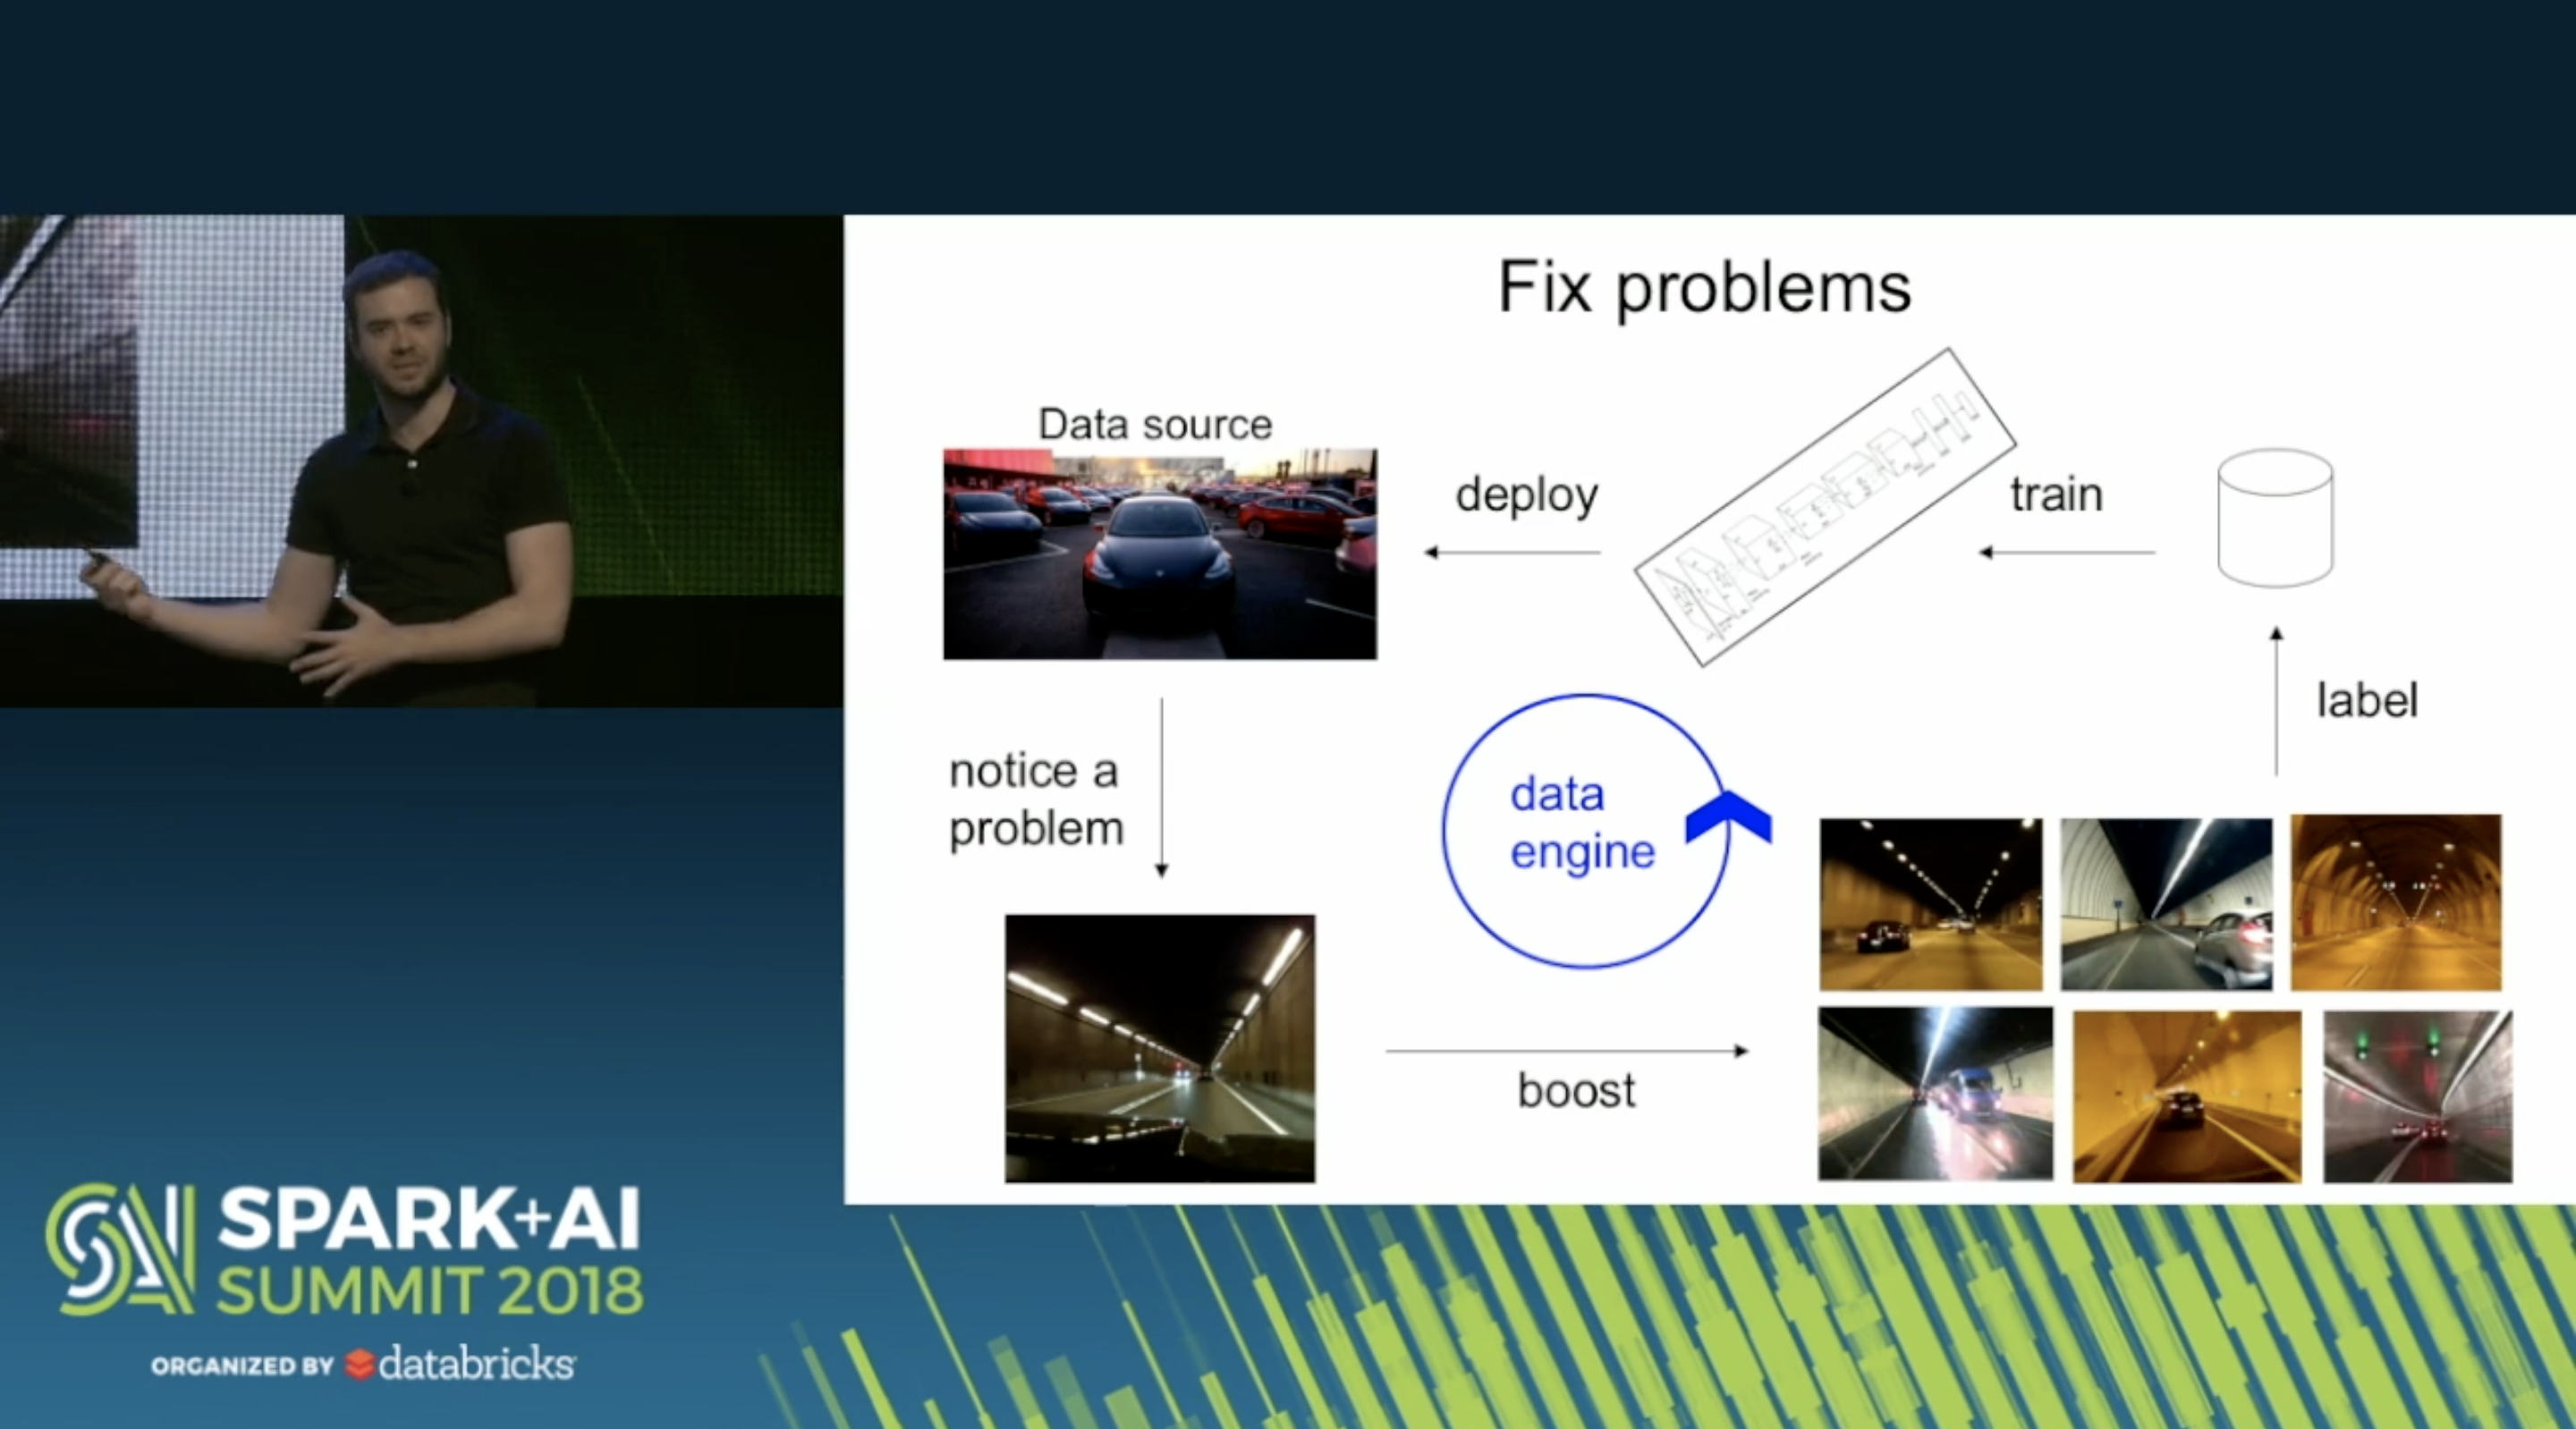
\includegraphics{images/spark-summit-karpathy-model-lifecycle.png}

\hypertarget{mlflow}{%
\subsection{MLflow}\label{mlflow}}

\begin{quote}
``Helps teams manage their machine learning lifecycle.''
\end{quote}

\begin{quote}
\begin{itemize}
\item
  \textbf{Tracking}

  : Track experiments to record and compare params and results.
\item
  \textbf{Projects}

  : Reuse and reproduce code to share or transfer to production.
\item
  \textbf{Models}

  : Manage and deploy models from across libraries and platforms.
\end{itemize}
\end{quote}

\hypertarget{what-is-r}{%
\section{What is R?}\label{what-is-r}}

\hypertarget{r-language}{%
\subsection{R Language}\label{r-language}}

\begin{quote}
R is a programming language and free software environment for
statistical computing and graphics.
\end{quote}

\begin{figure}

{\centering \includegraphics[width=500,height=300]{../../the-r-in-spark/images/01-intro-s-algorithm-interface} 

}

\caption{Interface language diagram by John Chambers - Rick Becker useR 2016.}\label{fig:unnamed-chunk-1}
\end{figure}

\hypertarget{r-community}{%
\subsection{R Community}\label{r-community}}

Provides a rich package archive provided in
\href{https://cran.r-project.org/}{CRAN} and
\href{https://www.bioconductor.org/}{Bioconductor}:
\href{https://CRAN.R-project.org/package=dplyr}{dplyr} to manipulate
data, \href{https://CRAN.R-project.org/package=cluster}{cluster} to
analyze clusters,
\href{https://CRAN.R-project.org/package=ggplot2}{ggplot2} to visualize
data, etc.

\begin{figure}

{\centering 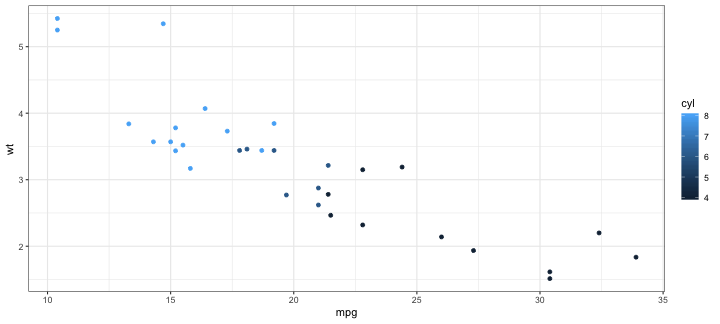
\includegraphics{slides_files/figure-latex/unnamed-chunk-2-1} 

}

\caption{Daily downloads of CRAN packages.}\label{fig:unnamed-chunk-2}
\end{figure}

\hypertarget{r-language-1}{%
\subsection{R Language}\label{r-language-1}}

Language features I would highlighting:

2.1.1 Vectors

2.1.4 Expression objects

2.1.8 Promise objects

2.1.9 Dot-dot-dot

3.1.4 Operators

\begin{quote}
\href{https://cran.r-project.org/doc/manuals/R-lang.html}{cran.r-project.org/doc/manuals/R-lang.html}
\end{quote}

\hypertarget{use-case}{%
\subsection{Use Case}\label{use-case}}

Select the \texttt{cyl} and \texttt{hp} columns and add 2 and 20:

\begin{Shaded}
\begin{Highlighting}[]
\NormalTok{mtcars}
\end{Highlighting}
\end{Shaded}

\begin{verbatim}
##                      mpg cyl  disp  hp drat    wt  qsec vs am gear carb
## Mazda RX4           21.0   6 160.0 110 3.90 2.620 16.46  0  1    4    4
## Mazda RX4 Wag       21.0   6 160.0 110 3.90 2.875 17.02  0  1    4    4
## Datsun 710          22.8   4 108.0  93 3.85 2.320 18.61  1  1    4    1
## Hornet 4 Drive      21.4   6 258.0 110 3.08 3.215 19.44  1  0    3    1
## Hornet Sportabout   18.7   8 360.0 175 3.15 3.440 17.02  0  0    3    2
## Valiant             18.1   6 225.0 105 2.76 3.460 20.22  1  0    3    1
## Duster 360          14.3   8 360.0 245 3.21 3.570 15.84  0  0    3    4
## Merc 240D           24.4   4 146.7  62 3.69 3.190 20.00  1  0    4    2
## Merc 230            22.8   4 140.8  95 3.92 3.150 22.90  1  0    4    2
## Merc 280            19.2   6 167.6 123 3.92 3.440 18.30  1  0    4    4
## Merc 280C           17.8   6 167.6 123 3.92 3.440 18.90  1  0    4    4
## Merc 450SE          16.4   8 275.8 180 3.07 4.070 17.40  0  0    3    3
## Merc 450SL          17.3   8 275.8 180 3.07 3.730 17.60  0  0    3    3
## Merc 450SLC         15.2   8 275.8 180 3.07 3.780 18.00  0  0    3    3
## Cadillac Fleetwood  10.4   8 472.0 205 2.93 5.250 17.98  0  0    3    4
## Lincoln Continental 10.4   8 460.0 215 3.00 5.424 17.82  0  0    3    4
## Chrysler Imperial   14.7   8 440.0 230 3.23 5.345 17.42  0  0    3    4
## Fiat 128            32.4   4  78.7  66 4.08 2.200 19.47  1  1    4    1
## Honda Civic         30.4   4  75.7  52 4.93 1.615 18.52  1  1    4    2
## Toyota Corolla      33.9   4  71.1  65 4.22 1.835 19.90  1  1    4    1
## Toyota Corona       21.5   4 120.1  97 3.70 2.465 20.01  1  0    3    1
## Dodge Challenger    15.5   8 318.0 150 2.76 3.520 16.87  0  0    3    2
## AMC Javelin         15.2   8 304.0 150 3.15 3.435 17.30  0  0    3    2
## Camaro Z28          13.3   8 350.0 245 3.73 3.840 15.41  0  0    3    4
## Pontiac Firebird    19.2   8 400.0 175 3.08 3.845 17.05  0  0    3    2
## Fiat X1-9           27.3   4  79.0  66 4.08 1.935 18.90  1  1    4    1
## Porsche 914-2       26.0   4 120.3  91 4.43 2.140 16.70  0  1    5    2
## Lotus Europa        30.4   4  95.1 113 3.77 1.513 16.90  1  1    5    2
## Ford Pantera L      15.8   8 351.0 264 4.22 3.170 14.50  0  1    5    4
## Ferrari Dino        19.7   6 145.0 175 3.62 2.770 15.50  0  1    5    6
## Maserati Bora       15.0   8 301.0 335 3.54 3.570 14.60  0  1    5    8
## Volvo 142E          21.4   4 121.0 109 4.11 2.780 18.60  1  1    4    2
\end{verbatim}

\hypertarget{how-to-not-write-r-code}{%
\subsection{How to NOT write R code}\label{how-to-not-write-r-code}}

This is how I would have written R code as a software engineer before
knowing R:

\begin{Shaded}
\begin{Highlighting}[]
\CommentTok{# Select columns subset}
\NormalTok{data =}\StringTok{ }\KeywordTok{data.frame}\NormalTok{(mtcars}\OperatorTok{$}\NormalTok{cyl, mtcars}\OperatorTok{$}\NormalTok{hp)}
\KeywordTok{colnames}\NormalTok{(data) =}\StringTok{ }\KeywordTok{c}\NormalTok{(}\StringTok{"cyl"}\NormalTok{, }\StringTok{"hp"}\NormalTok{)}

\CommentTok{# Transform each row}
\ControlFlowTok{for}\NormalTok{ (idx }\ControlFlowTok{in} \DecValTok{1}\OperatorTok{:}\KeywordTok{nrow}\NormalTok{(data)) \{}
\NormalTok{  data}\OperatorTok{$}\NormalTok{cyl[idx] =}\StringTok{ }\NormalTok{data}\OperatorTok{$}\NormalTok{cyl[idx] }\OperatorTok{+}\StringTok{ }\DecValTok{2}
\NormalTok{\}}

\CommentTok{# One column at a time to use the CPU cache efficiently}
\ControlFlowTok{for}\NormalTok{ (idx }\ControlFlowTok{in} \DecValTok{1}\OperatorTok{:}\KeywordTok{nrow}\NormalTok{(data)) \{}
\NormalTok{  data}\OperatorTok{$}\NormalTok{hp[idx] =}\StringTok{ }\NormalTok{data}\OperatorTok{$}\NormalTok{hp[idx] }\OperatorTok{+}\StringTok{ }\DecValTok{20}
\NormalTok{\}}
\end{Highlighting}
\end{Shaded}

\hypertarget{vectors}{%
\subsection{2.1.1 Vectors}\label{vectors}}

Everything is a vector in R:

\begin{Shaded}
\begin{Highlighting}[]
\CommentTok{# Select columns subset}
\NormalTok{data =}\StringTok{ }\KeywordTok{data.frame}\NormalTok{(mtcars}\OperatorTok{$}\NormalTok{cyl, mtcars}\OperatorTok{$}\NormalTok{hp)}
\KeywordTok{colnames}\NormalTok{(data) =}\StringTok{ }\KeywordTok{c}\NormalTok{(}\StringTok{"cyl"}\NormalTok{, }\StringTok{"hp"}\NormalTok{)}

\CommentTok{# Transform each row}
\NormalTok{data}\OperatorTok{$}\NormalTok{cyl =}\StringTok{ }\NormalTok{data}\OperatorTok{$}\NormalTok{cyl }\OperatorTok{+}\StringTok{ }\DecValTok{2}

\CommentTok{# One column at a time to use the CPU cache efficiently}
\NormalTok{data}\OperatorTok{$}\NormalTok{hp =}\StringTok{ }\NormalTok{data}\OperatorTok{$}\NormalTok{hp }\OperatorTok{+}\StringTok{ }\DecValTok{20}
\end{Highlighting}
\end{Shaded}

\hypertarget{dot-dot-dot}{%
\subsection{2.1.9 Dot-dot-dot}\label{dot-dot-dot}}

Dynamic parameters using the \texttt{...} parameter:

\begin{Shaded}
\begin{Highlighting}[]
\CommentTok{# Select columns subset}
\NormalTok{data =}\StringTok{ }\KeywordTok{data.frame}\NormalTok{(}\DataTypeTok{cyl =}\NormalTok{ mtcars}\OperatorTok{$}\NormalTok{cyl, }\DataTypeTok{hp =}\NormalTok{ mtcars}\OperatorTok{$}\NormalTok{hp)}

\CommentTok{# Transform each row}
\NormalTok{data}\OperatorTok{$}\NormalTok{cyl =}\StringTok{ }\NormalTok{data}\OperatorTok{$}\NormalTok{cyl }\OperatorTok{+}\StringTok{ }\DecValTok{2}

\CommentTok{# One column at a time to use the CPU cache efficiently}
\NormalTok{data}\OperatorTok{$}\NormalTok{hp =}\StringTok{ }\NormalTok{data}\OperatorTok{$}\NormalTok{hp }\OperatorTok{+}\StringTok{ }\DecValTok{20}
\end{Highlighting}
\end{Shaded}

\hypertarget{expression-and-promise-objects}{%
\subsection{2.1.4/2.1.8 Expression and Promise
objects}\label{expression-and-promise-objects}}

One can lazily evaluate operations and operate over expressions:

\begin{Shaded}
\begin{Highlighting}[]
\CommentTok{# Select columns subset}
\NormalTok{data =}\StringTok{ }\KeywordTok{select}\NormalTok{(mtcars, cyl, hp)}

\CommentTok{# Transform each row}
\NormalTok{data =}\StringTok{ }\KeywordTok{mutate}\NormalTok{(data, }\DataTypeTok{cyl =}\NormalTok{ cyl }\OperatorTok{+}\StringTok{ }\DecValTok{2}\NormalTok{)}

\CommentTok{# One column at a time to use the CPU cache efficiently}
\NormalTok{data =}\StringTok{ }\KeywordTok{mutate}\NormalTok{(data, }\DataTypeTok{hp =}\NormalTok{ hp }\OperatorTok{+}\StringTok{ }\DecValTok{20}\NormalTok{)}
\end{Highlighting}
\end{Shaded}

\hypertarget{operators}{%
\subsection{3.1.4 Operators}\label{operators}}

Use \texttt{\textless{}-} for assignment, or the newer
\texttt{\%\textgreater{}\%} pipe:

\begin{Shaded}
\begin{Highlighting}[]
\NormalTok{data <-}\StringTok{ }\NormalTok{mtcars }\OperatorTok\StringTok{ }
\StringTok{  }\KeywordTok{select}\NormalTok{(mtcars, cyl, hp) }\OperatorTok
\StringTok{  }\KeywordTok{mutate}\NormalTok{(data, }\DataTypeTok{cyl =}\NormalTok{ cyl }\OperatorTok{+}\StringTok{ }\DecValTok{2}\NormalTok{) }\OperatorTok
\StringTok{  }\KeywordTok{mutate}\NormalTok{(data, }\DataTypeTok{hp =}\NormalTok{ hp }\OperatorTok{+}\StringTok{ }\DecValTok{20}\NormalTok{)}
\end{Highlighting}
\end{Shaded}

\hypertarget{linear-models}{%
\subsection{Linear Models}\label{linear-models}}

\begin{Shaded}
\begin{Highlighting}[]
\KeywordTok{lm}\NormalTok{(mpg }\OperatorTok{~}\StringTok{ }\NormalTok{cyl }\OperatorTok{+}\StringTok{ }\NormalTok{hp, mtcars) }\OperatorTok\StringTok{ }\KeywordTok{plot}\NormalTok{()}
\end{Highlighting}
\end{Shaded}

\hypertarget{mlflow-with-r}{%
\section{MLflow with R}\label{mlflow-with-r}}

\hypertarget{principles}{%
\subsection{Principles}\label{principles}}

\begin{itemize}
\tightlist
\item
  Parity with Python API.
\item
  Designed for the R user.
\end{itemize}

\hypertarget{installing}{%
\subsection{Installing}\label{installing}}

\begin{quote}
Install Anaconda or miniconda.
\end{quote}

Today\ldots{}

\begin{Shaded}
\begin{Highlighting}[]
\FunctionTok{git}\NormalTok{ clone https://github.com/mlflow/mlflow}
\end{Highlighting}
\end{Shaded}

\begin{Shaded}
\begin{Highlighting}[]
\NormalTok{devtools}\OperatorTok{::}\KeywordTok{install_github}\NormalTok{(}\StringTok{"mlflow/mlflow"}\NormalTok{, }\DataTypeTok{subdir =} \StringTok{"R/mlflow"}\NormalTok{)}

\NormalTok{mlflow}\OperatorTok{::}\KeywordTok{mlflow_install}\NormalTok{()}

\NormalTok{reticulate}\OperatorTok{::}\KeywordTok{conda_install}\NormalTok{(}\StringTok{"r-mlflow"}\NormalTok{, }\StringTok{"<local github repo>"}\NormalTok{, }\DataTypeTok{pip =} \OtherTok{TRUE}\NormalTok{)}
\end{Highlighting}
\end{Shaded}

Soon\ldots{}

\begin{Shaded}
\begin{Highlighting}[]
\KeywordTok{install.packages}\NormalTok{(}\StringTok{"mlflow"}\NormalTok{)}
\NormalTok{mlflow}\OperatorTok{::}\KeywordTok{mlflow_install}\NormalTok{()}
\end{Highlighting}
\end{Shaded}

\hypertarget{tracking---implicit}{%
\subsection{Tracking - Implicit}\label{tracking---implicit}}

Implicit MLflow run:

\begin{Shaded}
\begin{Highlighting}[]
\KeywordTok{library}\NormalTok{(mlflow)}

\CommentTok{# Log a parameter (key-value pair)}
\KeywordTok{mlflow_log_param}\NormalTok{(}\StringTok{"param1"}\NormalTok{, }\DecValTok{5}\NormalTok{)}

\CommentTok{# Log a metric; metrics can be updated throughout the run}
\KeywordTok{mlflow_log_metric}\NormalTok{(}\StringTok{"foo"}\NormalTok{, }\DecValTok{1}\NormalTok{)}
\KeywordTok{mlflow_log_metric}\NormalTok{(}\StringTok{"foo"}\NormalTok{, }\DecValTok{2}\NormalTok{)}
\KeywordTok{mlflow_log_metric}\NormalTok{(}\StringTok{"foo"}\NormalTok{, }\DecValTok{3}\NormalTok{)}

\CommentTok{# Log an artifact (output file)}
\KeywordTok{writeLines}\NormalTok{(}\StringTok{"Hello world!"}\NormalTok{, }\StringTok{"output.txt"}\NormalTok{)}
\KeywordTok{mlflow_log_artifact}\NormalTok{(}\StringTok{"output.txt"}\NormalTok{)}
\end{Highlighting}
\end{Shaded}

Run terminates when the R session finishes or by running:

\begin{Shaded}
\begin{Highlighting}[]
\KeywordTok{mlflow_end_run}\NormalTok{()}
\end{Highlighting}
\end{Shaded}

Useful when sourcing files.

\hypertarget{tracking---explicit}{%
\subsection{Tracking - Explicit}\label{tracking---explicit}}

Explicit MLflow run:

\begin{Shaded}
\begin{Highlighting}[]
\KeywordTok{library}\NormalTok{(mlflow)}

\KeywordTok{with}\NormalTok{(}\KeywordTok{mlflow_start_run}\NormalTok{(), \{}
  \CommentTok{# Log a parameter (key-value pair)}
  \KeywordTok{mlflow_log_param}\NormalTok{(}\StringTok{"param1"}\NormalTok{, }\DecValTok{5}\NormalTok{)}
  
  \CommentTok{# Log a metric; metrics can be updated throughout the run}
  \KeywordTok{mlflow_log_metric}\NormalTok{(}\StringTok{"foo"}\NormalTok{, }\DecValTok{1}\NormalTok{)}
  \KeywordTok{mlflow_log_metric}\NormalTok{(}\StringTok{"foo"}\NormalTok{, }\DecValTok{2}\NormalTok{)}
  \KeywordTok{mlflow_log_metric}\NormalTok{(}\StringTok{"foo"}\NormalTok{, }\DecValTok{3}\NormalTok{)}
  
  \CommentTok{# Log an artifact (output file)}
  \KeywordTok{writeLines}\NormalTok{(}\StringTok{"Hello world!"}\NormalTok{, }\StringTok{"output.txt"}\NormalTok{)}
  \KeywordTok{mlflow_log_artifact}\NormalTok{(}\StringTok{"output.txt"}\NormalTok{)}
\NormalTok{\})}
\end{Highlighting}
\end{Shaded}

\hypertarget{tracking---sources}{%
\subsection{Tracking - Sources}\label{tracking---sources}}

\begin{Shaded}
\begin{Highlighting}[]
\KeywordTok{mlflow_run}\NormalTok{(}\StringTok{"R/tracking.R"}\NormalTok{)}
\end{Highlighting}
\end{Shaded}

Or adding the following to \texttt{tracking.R} in RStudio 1.2:

\begin{Shaded}
\begin{Highlighting}[]
\CommentTok{# !source mlflow::mlflow_run(entry_point = .file)}
\end{Highlighting}
\end{Shaded}

\hypertarget{tracking---ui}{%
\subsection{Tracking - UI}\label{tracking---ui}}

\begin{Shaded}
\begin{Highlighting}[]
\KeywordTok{mlflow_ui}\NormalTok{()}
\end{Highlighting}
\end{Shaded}

\hypertarget{projects---snapshots}{%
\subsection{Projects - Snapshots}\label{projects---snapshots}}

Create dependencies snapshot:

\begin{Shaded}
\begin{Highlighting}[]
\KeywordTok{mlflow_snapshot}\NormalTok{()}
\end{Highlighting}
\end{Shaded}

Then restore snapshot:

\begin{Shaded}
\begin{Highlighting}[]
\KeywordTok{mlflow_restore_snapshot}\NormalTok{()}
\end{Highlighting}
\end{Shaded}


\includegraphics{images/r-package-packrat.png}

\hypertarget{projects---consuming}{%
\subsection{Projects - Consuming}\label{projects---consuming}}

\begin{Shaded}
\begin{Highlighting}[]
\KeywordTok{mlflow_run}\NormalTok{(}
  \StringTok{"train.R"}\NormalTok{,}
  \StringTok{"https://github.com/rstudio/mlflow-example"}\NormalTok{,}
  \DataTypeTok{param_list =} \KeywordTok{list}\NormalTok{(}\DataTypeTok{alpha =} \FloatTok{0.2}\NormalTok{)}
\NormalTok{)}
\end{Highlighting}
\end{Shaded}

\begin{verbatim}
Elasticnet model (alpha=0.2, lambda=0.5):
  RMSE: 0.827574750159859
  MAE: 0.632070002076146
  R2: 0.227227498131926
\end{verbatim}

Or from bash:

\begin{Shaded}
\begin{Highlighting}[]
\ExtensionTok{mlflow}\NormalTok{ run --entry-point train.R https://github.com/rstudio/mlflow-example}
\end{Highlighting}
\end{Shaded}

\hypertarget{models---saving}{%
\subsection{Models - Saving}\label{models---saving}}

\begin{Shaded}
\begin{Highlighting}[]
\KeywordTok{mlflow_save_model}\NormalTok{(model)}
\end{Highlighting}
\end{Shaded}

Generic functions are serialized with \texttt{crate}:

\begin{Shaded}
\begin{Highlighting}[]
\NormalTok{column <-}\StringTok{ }\KeywordTok{mlflow_log_param}\NormalTok{(}\StringTok{"column"}\NormalTok{, }\DecValTok{1}\NormalTok{)}
\NormalTok{model <-}\StringTok{ }\KeywordTok{lm}\NormalTok{(}
\NormalTok{  Sepal.Width }\OperatorTok{~}\StringTok{ }\NormalTok{x,}
  \KeywordTok{data.frame}\NormalTok{(}\DataTypeTok{Sepal.Width =}\NormalTok{ iris}\OperatorTok{$}\NormalTok{Sepal.Width, }\DataTypeTok{x =}\NormalTok{ iris[,column])}
\NormalTok{)}

\KeywordTok{mlflow_save_model}\NormalTok{(}
  \KeywordTok{crate}\NormalTok{(}\OperatorTok{~}\StringTok{ }\NormalTok{stats}\OperatorTok{::}\KeywordTok{predict}\NormalTok{(model, .x), model)}
\NormalTok{)}
\end{Highlighting}
\end{Shaded}

However, \texttt{mlflow\_save\_model()} can be extended by packages:

\begin{Shaded}
\begin{Highlighting}[]
\CommentTok{#' @export}
\NormalTok{mlflow_save_flavor.tensorflow <-}\StringTok{ }\ControlFlowTok{function}\NormalTok{(...) \{\}}
\NormalTok{mlflow_load_flavor.tensorflow <-}\StringTok{ }\ControlFlowTok{function}\NormalTok{(...) \{\}}
\NormalTok{mlflow_predict_flavor.tensorflow <-}\StringTok{ }\ControlFlowTok{function}\NormalTok{(...) \{\}}
\end{Highlighting}
\end{Shaded}

\hypertarget{models---predictions}{%
\subsection{Models - Predictions}\label{models---predictions}}

\begin{Shaded}
\begin{Highlighting}[]
\KeywordTok{mlflow_rfunc_predict}\NormalTok{(}
  \StringTok{"model"}\NormalTok{,}
  \DataTypeTok{data =} \KeywordTok{data.frame}\NormalTok{(}\DataTypeTok{x =} \KeywordTok{c}\NormalTok{(}\FloatTok{0.3}\NormalTok{, }\FloatTok{0.2}\NormalTok{))}
\NormalTok{)}
\end{Highlighting}
\end{Shaded}

\begin{verbatim}
       1        2 
3.400381 3.406570
\end{verbatim}

Or from bash,

\begin{Shaded}
\begin{Highlighting}[]
\ExtensionTok{mlflow}\NormalTok{ rfunc predic --model-path model --input-path data.csv}
\end{Highlighting}
\end{Shaded}

\hypertarget{models---serving}{%
\subsection{Models - Serving}\label{models---serving}}

\begin{Shaded}
\begin{Highlighting}[]
\KeywordTok{mlflow_rfunc_serve}\NormalTok{(}\StringTok{"model"}\NormalTok{)}
\end{Highlighting}
\end{Shaded}

\begin{Shaded}
\begin{Highlighting}[]
\ExtensionTok{mlflow}\NormalTok{ rfunc serve model-path model}
\end{Highlighting}
\end{Shaded}

\begin{Shaded}
\begin{Highlighting}[]
\ExtensionTok{curl}\NormalTok{ -X POST }\StringTok{"http://127.0.0.1:8090/predict/"}\NormalTok{ -H }\StringTok{"accept: application/json"}\NormalTok{ -H }\StringTok{"Content-Type: application/json"}\NormalTok{ -d }\StringTok{'[\{"x": [0.3, 0.2]\}]'}
\end{Highlighting}
\end{Shaded}

\hypertarget{future-work}{%
\subsection{Future Work}\label{future-work}}

Currently merged, various github issues pending:

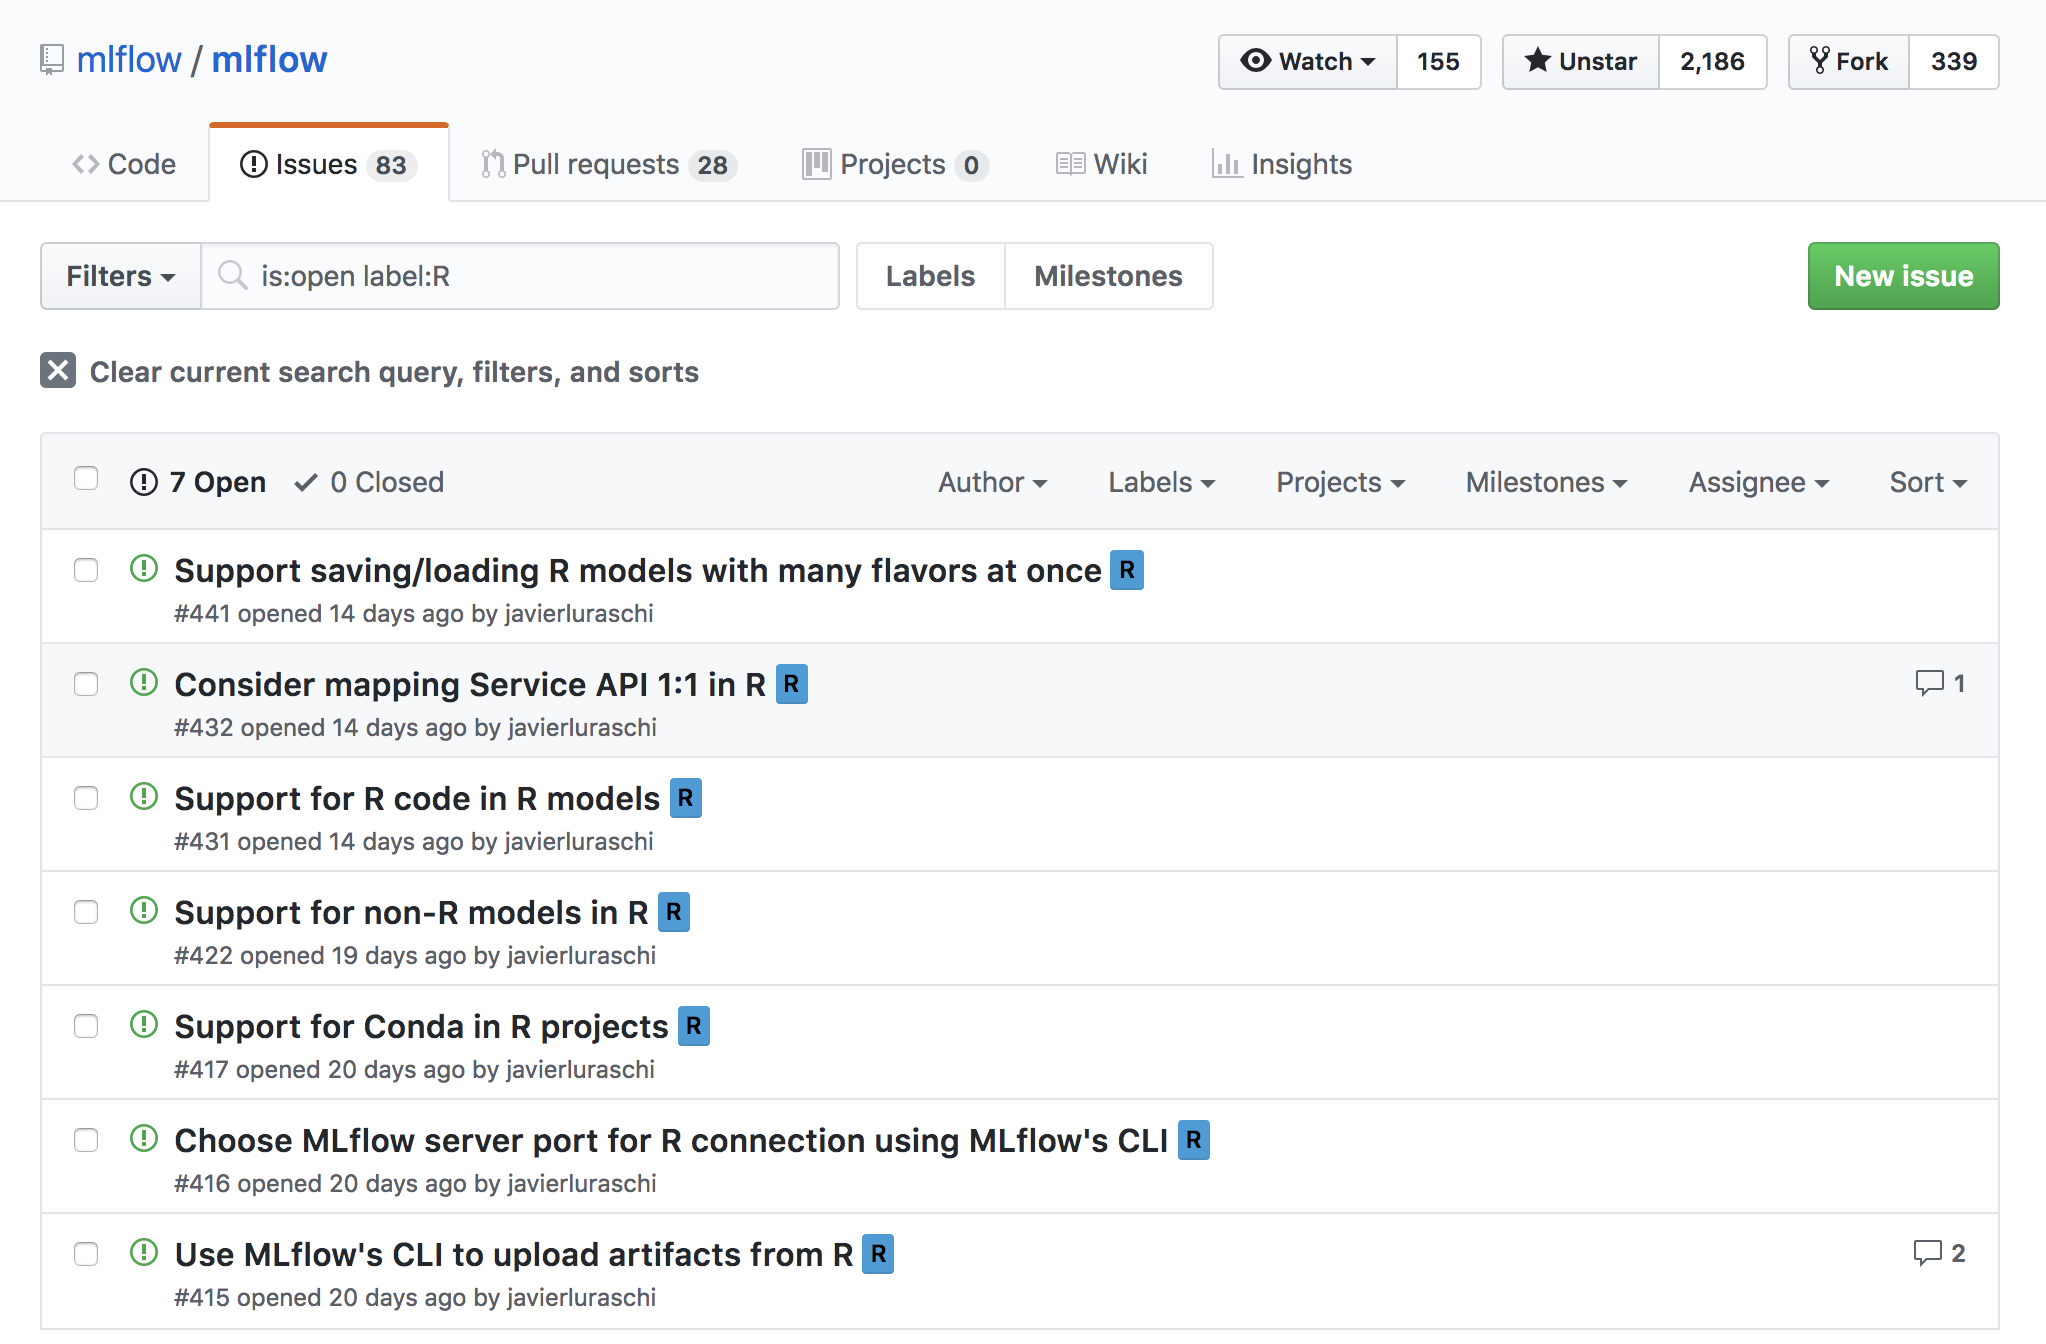
\includegraphics{images/mlflow-github-r-issues.png}

\hypertarget{thanks}{%
\subsection{Thanks!}\label{thanks}}

\begin{quote}
github.com/mlflow/mlflow
\end{quote}

\begin{quote}
@javierluraschi
\end{quote}

\begin{quote}
\href{mailto:javier@rstudio.com}{\nolinkurl{javier@rstudio.com}}
\end{quote}


\end{document}
